\documentclass[ignorenonframetext]{beamer}
%\usetheme{Boadilla}
\usetheme{PaloAlto}
%\usetheme{Berlin}
%\usecolor{}

\mode<presentation>

\usepackage{minted}


\usepackage{xcolor}
\usepackage{colortbl}

\usepackage{fontspec}
\setmainfont{Linux Libertine O}
\usepackage{xltxtra}
\usepackage[english,french]{babel}

\usepackage{framed}
\definecolor{shadecolor}{gray}{0.95}
\usepackage{longtable}
\usepackage[normalem]{ulem}

\usepackage{tikz}

\institute{École nationale des chartes | Paris, Sciences \& Lettres}

\title{Philologie numérique: constituer un corpus}
\subtitle{Atelier \textit{Humanités numériques}}
\author{Jean-Baptiste Camps}
\date[Madrid, 9 oct. 2018]{Casa de Velázquez\\ Madrid, 9 octobre 2018}

\makeatletter 
         
        \AtBeginSection[]{% 
        \begin{frame}{Plan}%
        \small
        \tableofcontents[currentsection]%
        \end{frame} }

        %\AtBeginSubsection[]{% 
	%\begin{frame}{Plan}%
	%\small
	%\tableofcontents[currentsection,currentsubsection]%
%\end{frame} }


\makeatother 
    
    
\begin{document}

\frame{\maketitle}



\begin{frame}{Acquisition du texte}

Dans la constitution d'un corpus de textes, la première phase est bien sûr l'acquisition du contenu des textes envisagés.
\begin{description}
	\item[Transcription] des témoins, selon les critères scientifiques du projet (transcriptions allographétiques, graphématiques, normalisées; édition critique; etc.). Méthode souvent la plus sûre, mais aussi la plus lente;
	\item[``Transcription'' assistée par ordinateur] en utilisant un algorithme permettant la reconnaissance optique de caractères (\textit{optical character recognition} ou \textsc{ocr}) imprimés, ou la reconnaissance des écritures manuscrites (\textit{handwritten text recognition} ou \textsc{htr}).
	\item[Téléchargement] de textes depuis des corpus en lignes, des sites d'édition électronique, des bases de données d'éditeurs, etc.
\end{description}

\end{frame}


\begin{frame}{Reconnaissance des écritures manuscrites}

\begin{columns}
\begin{column}{0.48\textwidth}
	Reconnaissance optique des caractères (imprimés)\\
	\textit{Optical character recognition} (\textsc{ocr})
	\begin{itemize}
		\item ``problème résolu'' de l'informatique;
		\item aisé d'obtenir des taux d'erreur caractère (CER) < 2\%;
		\item outils libres: \texttt{Tesseract} 4, …;
		\item existence de modèles génériques (par langue).
	\end{itemize}
\end{column}
\begin{column}{0.48\textwidth}
	Reconnaissance des écritures manuscrites\\
	\textit{Handwritten text recognition} (\textsc{htr})
	\begin{itemize}
		\item très peu fonctionnel jusqu'à ces dernières années;
		\item nouveaux développements: IA (réseaux de neurone récurrents LSTM…);
		\item outils libres: \texttt{OCRopy}, …
		\item modèles spécifiques à entraîner (pour chaque main, écriture,…).
	\end{itemize}
\end{column}
\end{columns}

\end{frame}

%Mesure d'erreur: character error rate (CER)
%etc.

%Éléments à reprendre:
% - article Albi
% - projet CNRS


\begin{frame}{Les étapes}
\begin{enumerate}
\item traitement des images;
\item analyse de la mise en page et identification des lignes;
\item reconnaissance des caractères;
\item d'éventuels post-traitements, visant à améliorer les résultats.
\end{enumerate}
\end{frame}

%Les outils: 
% Outils spécifiques aux données patrimoniales
%   - Oriflamms
%   - Transkribus

% Outils généralistes
%   - OCRopy / CLSTM
%   - OCRopy 2
%   - Tesseract 4

\section{Un outil ``tout en un'': \texttt{Transkribus}}

\begin{frame}{Transkribus}

\begin{columns}
\begin{column}{0.45\textwidth}
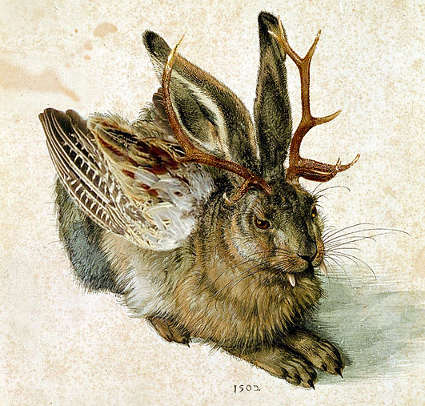
\includegraphics[width=\textwidth]{img/wolpertinger.jpg}
\end{column}
\begin{column}{0.45\textwidth}
\begin{itemize}
\item développé par un consortium de recherche européen (projet \textsc{read}; Univ. Innsbruck et al.);
\item financé par la Commission Européenne (Horizon 2020);
\item permet de charger des images, analyser la mise en page, segmenter…
\item opérations réalisées sur les \alert{serveurs de Transkribus}.
\end{itemize}
\end{column}
\end{columns}

\end{frame}

\begin{frame}{Installer Transkribus}

\begin{itemize}
\item Se rendre sur: \url{https://transkribus.eu/Transkribus/};
\item se connecter (ou créer un compte) et télécharger le logiciel;
\item extraire l'archive;
\item lancer le logiciel (\texttt{Transkribus.sh} ou \texttt{Transkribus.exe});
\item tutoriel: \url{https://transkribus.eu/wiki/images/7/77/How_to_use_TRANSKRIBUS_-_10_steps.pdf};
\item wiki: \url{https://transkribus.eu/wiki/index.php/Main_Page}.
\end{itemize}


\end{frame}

\begin{frame}[shrink]
\frametitle{T.P. Transkribus}

\begin{enumerate}
\item se connecter;
\item importer un document (choisir un ou deux fol. du dossier Cid ou \texttt{digby\_23});
\item lancer l'analyse de la mise en page;
\item corriger la segmentation
\begin{itemize}
\item régions de texte, 
\item zone de ligne, 
\item ligne de référence, 
\item mots,…;
\end{itemize}
si besoin en
\begin{itemize}
\item étendant le rectangle;
\item déplaçant les points.
\end{itemize}
\item[] N.B.: il est possible de choisir les types de zone que l'on veut afficher ou non;
\item océriser / commencer à transcrire;
\item ajouter quelques balises et compléter quelques métadonnées;
\item sauvegarder la transcription;
\item consulter la source;
\item exporter le document en \textsc{tei} (attention au ``tag abuse'' de l'export par défaut).
\end{enumerate}

\end{frame}

\section{Pas-à-pas avec ScanTailor et OCRopy}

\subsection{Traitement des images}

\begin{frame}{}
\begin{columns}
\begin{column}{0.45\textwidth}
Dans une démarche de reconnaissance des écritures, la qualité des images
et de leurs traitements est cruciale.
\end{column}
\begin{column}{0.45\textwidth}
Besoins:
\begin{enumerate}
\item images en 300 DPI;
\item redressées, débruitées;
\item binarisées.
\end{enumerate}
Outils: logiciels de traitement d'image, par ex. \texttt{ScanTailor}
\end{column}
\end{columns}

\end{frame}

\begin{frame}{T.P. ScanTailor}

\begin{enumerate}
\item Démarrer un nouveau projet;
\item charger les images du dossier \texttt{digby\_23};
\item suivre les différentes étapes dans le logiciel;
\item exporter en tiff binarisé 300 DPI.
\end{enumerate}

\end{frame}

\subsection{Analyse de la mise en page}

%TODO: Divadia, autres algos
\begin{frame}{Analyser la mise en page}
\begin{columns}
\begin{column}{0.45\textwidth}
\textbf{Identifier}
\begin{itemize}
\item zones de texte;
\item décoration;
\item colonnes;
\item lignes;
\item mots;
\item lettres.
\end{itemize}
\end{column}
\begin{column}{0.45\textwidth}
\textbf{Approches}
\begin{itemize}
\item Sans apprentissage, par ex.
\begin{itemize}
\item \texttt{OCRopy} 1;
\item \textsc{Oriflamms} (\textsc{IRHT});
\end{itemize}
\item fondée sur des méthodes d'apprentissage (IA), par ex.
\begin{itemize}
\item \texttt{OCRopy} 2?
\end{itemize}
\end{itemize}
\end{column}
\end{columns}

\end{frame}

\begin{frame}[fragile]
\frametitle{Installer OCRopy}

\begin{minted}{bash}
$ git clone https://github.com/tmbdev/ocropy.git
$ cd ocropy
$ virtualenv ocropus_venv/
$ source ocropus_venv/bin/activate
$ pip install -r requirements.txt
$ python setup.py install
\end{minted}

\end{frame}

\begin{frame}[fragile]
\frametitle{Analyser la mise en page avec \texttt{OCRopy}}
Depuis la racine du dossier:
\begin{minted}{bash}
#Binarisation
$ ./ocropy/ocropus-nlbin tif/* -o book
#Segmentation en lignes
$ ./ocropy/ocropus-gpageseg -n book/*.bin.png	
\end{minted}

Vérifier la qualité du résultat.

\end{frame}


\subsection{Reconnaissance des écritures manuscrites}

\begin{frame}
\frametitle{Différentes solutions techniques}

%Différents outils de ROC/ROM, et paradigmes techniques
%Lequel est le plus adapté, choix d'Ocropy/CLSTM

\begin{itemize}
\item approches segmentées ou non segmentées;
\item mesures de distance; méthodes statistiques (chaînes de Markov) ou d'intelligence artificielle (réseaux de neurones convolutifs ou récurrents, LSTM 1D, LSTM 2D, etc.);
\item outils directement opérationnels ou nécessitant un entraînement.
\end{itemize}

%	\pause

\begin{block}{Ocropy et CLSTM}
Outils développés par Thomas M. Breuel (\url{https://github.com/tmbdev/ocropy}; \url{http://github.com/tmbdev/clstm}).
\begin{itemize}
\item approche non segmentées;
\item réseaux de neurones récurrents (LSTM);
\item \textit{open source} et nécessitant l'entraînement d'un modèle.
\end{itemize}
\end{block}

\end{frame}


\begin{frame}[fragile]
\frametitle{Ocropy: un apprentissage guidé}

\only<1>{

\centering
\begin{tikzpicture}
\node[draw, rectangle, rounded corners=3pt] (P) at (-4,6)
{Prétraitement des images};%
\node[draw, rectangle, rounded corners=3pt] (A) at (-3,5)
{Analyse mise en page};%
\node[draw, rectangle, rounded corners=3pt] (GT) at (0,2.5)
{Vérité de terrain};
\node[draw, rectangle, rounded corners=3pt] (T) at (4,2.5)
{Entraînement};
\node[draw, rectangle, rounded corners=3pt] (TT) at (2,0)
{Test};
\node[draw, rectangle, rounded corners=3pt] (O) at (2,-1)
{Sortie};

\draw[->,>=latex] (P) -- (A) ;
\draw[->,>=latex] (A) -- (GT) node[midway,sloped,above] {transcription}; 
\draw[->,>=latex] (GT) -- (T) ; 
\draw[->,>=latex] (T) -- (TT) ;
\draw[->,>=latex] (TT) -- (GT) node[midway,sloped,above] {relecture};
\draw[->,>=latex] (TT) -- (O) ;
\end{tikzpicture}

} 


\only<2>{
\begin{block}{Déclaration de caractères}
\centering
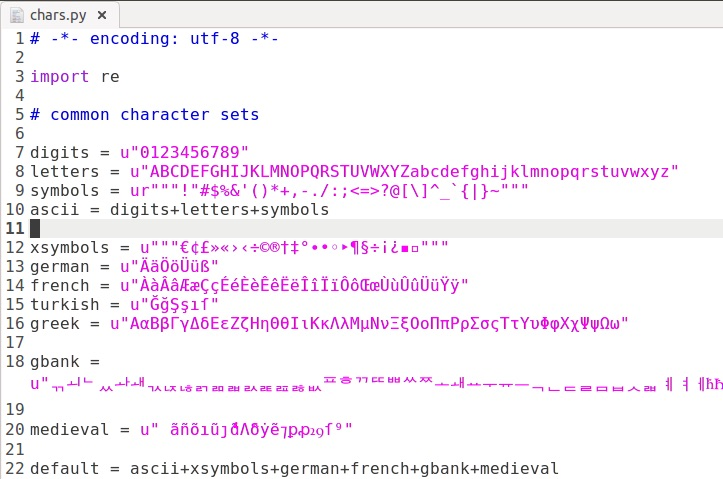
\includegraphics[width=0.8\textwidth]{img/chars-py.jpg}

\footnotesize{NB: avec CLSTM, cette étape n'est plus nécessaire.}
\end{block}

\alert{Copier le fichier \texttt{chars.py} qui se trouve à la racine
du dossier à la place de celui qui se trouve dans \texttt{ocrolib}.
}
}


\only<3>{
\begin{block}{Entraînement sur un ms. (ici Roland d'Oxford)}\centering
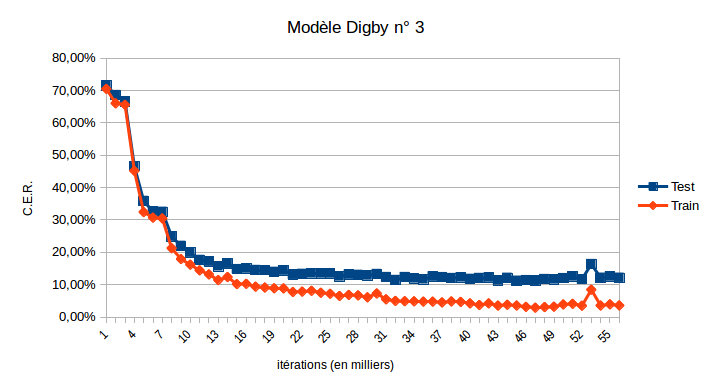
\includegraphics[width=\textwidth]{img/entrainementDigby3.png}

\end{block}
}

\only<4>{
\begin{block}{Test}\centering
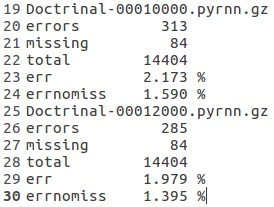
\includegraphics[width=0.4\linewidth]{img/test.jpg}
\hfill
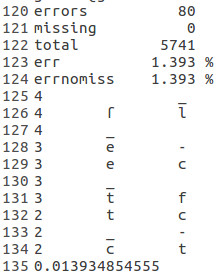
\includegraphics[width=0.3\linewidth]{img/econf.jpg}
\end{block}
}

\only<5>{
\begin{block}{Résultats}
\begin{itemize}
\item pour un imprimé ancien, des taux d'erreur de l'ordre de 1\% sont atteignables…
\item pour un ms., des taux inférieurs à 10\% sont atteignables avec seulement 400 lignes d'entraînement environ (cas du Digby 23, jusqu'à 7\% de CER).
\end{itemize}
\end{block}
}

\end{frame}

\begin{frame}[fragile]

\frametitle{Confusions fréquentes (ms.)}

\begin{verbatim}
digby4/test3-138000.clstm
errors         193
missing          0
total        14767
err          1.307 %
errnomiss    1.307 %
25  s  S
17  _  .
14     _
\end{verbatim}

\end{frame}

\begin{frame}[fragile]
\frametitle{T.P. \texttt{OCRopy}: Préparation des données}

\textbf{1. Essayer d'appliquer un modèle déjà entraîné}
\begin{minted}{bash}
#Lancer la reconnaissance
$ ./ocropy/ocropus-rpred -n -m 
./ocropy/models/digby23-00106000.pyrnn.gz 
book/*/*.bin.png
#Extraire le résultat
$ ./ocropy/ocropus-gtedit html -H35 
book/*/*.bin.png -o gt.html
\end{minted}

Pas terrible… Mais comment améliorer le modèle?

\textbf{2. Corriger / transcrire}
\end{frame}

\begin{frame}[fragile]
\frametitle{T.P. \texttt{OCRopy}: Entraînement}


\textbf{3. Extraire et entraîner}
\begin{minted}{bash}
#Extraire
$ ./ocropy/ocropus-gtedit extract gt.html
#Normalisation des caractères
$ for f in book/*/*.gt.txt; do uconv -f utf8 -t utf8 
-x nfc -o "${f/gt.txt/gtneu.txt}" "$f"; done
$for f in book/*/*.gtneu.txt; do mv "$f" 
"${f/gtneu.txt/gt.txt}"; done
\end{minted}
Puis placer 90\% des lignes corrigées dans un dossier \texttt{train} et 10\% dans un dossier \texttt{test}.\\
On peut ensuite lancer un entraînement (de zéro ou à partir du modèle précédent, aux choix). 
\begin{minted}{bash}
#Lancer l'entraînement
$ ./ocropy/ocropus-rtrain -o digby 
-d 1 train/*/*.bin.png
\end{minted}

\end{frame}

\begin{frame}[fragile]
\frametitle{T.P. \texttt{OCRopy}: Test des résultats}


\textbf{4. Tester les résultats}

Une fois que l'entraînement a atteint un niveau satisfaisant, on peut tester la qualité du résultat, 

\begin{minted}{bash}
# Calcul des erreurs de différents modèles, comparativement
for i in *.pyrnn.gz; do 
echo "$i" >> modeltest 
./ocropy/ocropus-rpred -n -m $i test/*/*.bin.png
./ocropy/ocropus-errs test/*/*.gt.txt 2>>modeltest 
done
# Confusions de caractères
./ocropy/ocropus-econf test/*/*.gt.txt
\end{minted}

\end{frame}


\end{document}